\chapter{Cloud-Native Patterns in der Anwendungsarchitektur}

In der entwickelten Cloud-Native-Anwendung zur Beratung für nachhaltige Energiegewinnungsstandorte finden sich verschiedene Cloud-Native Patterns. Nachfolgend werden die verwendeten Pattern "Microservices Architecture" und "Communicate Through APIs" aus dem Bereich "Development \& Design" sowie die Pattern "Continuous Delivery" und "Continuous Deployment" aus dem Bereich "Infrastructure \& Cloud" vorgestellt, die beide jeweils eng miteinander verknüpft sind.

\subsection{1. Microservices Architecture \& Communicate Through APIs (Development \& Design)}

Die Anwendung folgt dem Pattern der \textbf{Microservices-Architektur}, bei dem die Gesamtanwendung in mehrere unabhängige, spezialisierte Services unterteilt wird, um Kosten für die Koordination zwischen Teams zu senken. \cite{MicroservicesArchitecture}

Eng damit verbunden ist die Kommunikation mit den entsprechenden Microservices. Diese läuft über stabile und voneinander getrennte APIs, was dem Pattern \textbf{Communicate Through APIs} entspricht. \cite{CommunicateThroughAPIs}.

In der vorliegenden Anwendung gibt es beispielsweise den \textbf{Weather-Microservice}, der für die Verarbeitung und Bereitstellung von Wetterdaten zuständig ist, und den \textbf{Geo-Microservice}, der Informationen zur geographischen Infrastruktur bereitstellt.
\textbf{Weather-Microservice:} Dieser Service ist verantwortlich für die Verarbeitung und Bereitstellung von Wetterdaten. Er bezieht seine Informationen über die OpenMeteo-APIs, die sowohl historische als auch aktuelle Wetterbedingungen bereitstellen. Die Wetterdaten werden in einer PostgreSQL-Datenbank gespeichert, um eine effiziente Abfrage und Analyse zu ermöglichen. Zudem beinhaltet der Weather-Microservice ein Modell zur Wettervorhersage, das auf historischen Wetterdaten basiert und Prognosen für zukünftige Wetterbedingungen erstellt.

\textbf{Geo-Microservice:} Der Geo-Microservice liefert Informationen zur vorherrschenden Infrastruktur, einschließlich der Überprüfung der Entfernung zu bestehenden Stromleitungen und der Lage in Bezug auf Naturschutzgebiete, Wald oder Wohngebiete. Die Daten für diesen Service werden aus der Overpass-API von OpenStreetMap bezogen.\\

Beide Microservices sind über REST-APIs erreichbar und in Containern isoliert, was eine flexible und skalierbare Architektur gewährleistet.

\textbf{Vorteile des Einsatzes:} 
Die Microservices-Architektur ermöglicht eine modulare Entwicklung, bei der unterschiedliche Teammitglieder an den Komponenten der Anwendung parallel arbeiten können. Die Entwicklung des Weather-Microservice erfolgte beispielsweise separat von der des Geo-Microservices. Dies ermöglicht eine höhere Agilität der Entwicklung und erhöht die Entwicklungsgeschwindigkeit. Zudem kann jeder Microservice die für ihn am besten geeigneten Technologien verwenden, was die Effizienz und Leistung der jeweiligen Anwendung verbessert. Der Weather-Microservice nutzt beispielsweise eine PostgreSQL-Datenbank zur Speicherung der Wetterdaten. Würde der Geo-Service auch eine Datenbank benötigen, könnte er eine PostgreSQL-Datenbank mit PostGIS-Erweiterung nutzen, welche speziell für räumliche Datentypen gedacht ist und eine einfachere Suche nach Orten innerhalb des Suchradius ermöglicht. Diese Erweiterung wäre für den Weather-Microservice nicht benötigt.\\

Eng mit der Verwendung der Microservices wird bei der hier vorliegenden Anwendung auch das Pattern \textbf{Communicate Through APIs} genutzt. Alle Interaktionen zwischen dem Frontend und dem Weather- sowie dem Geo-Microservice erfolgen über klar definierte REST-APIs. Dies trägt ebenso positiv zur Wartbarkeit und Flexibilität der Anwendung bei. Wenn beispielsweise der Geo-Microservice überearbeitet werden muss, bleibt das Frontend unberührt, solange die API-Schnittstelle beibehalten wird.

\subsection{2. Continuous Delivery und Continuous Deployment (Infrastructure \& Cloud)}

Ein zentrales Pattern in der Anwendungsarchitektur ist \textbf{ContinuousDelivery}, das einen schnellen Programmier-, Test- und Auslieferungszyklus ermöglicht. Dies erlaubt es, neue Funktionen zügig zu veröffentlichen und schnell auf Benutzerfeedback zu reagieren \cite{ContinuousDelivery}. Eng verknüpft mit diesem Pattern ist das \textbf{ContinuousDeployment}, das sicherstellt, dass jede Änderung, die den Testprozess besteht, automatisch in die Produktionsumgebung überführt wird. Dies sorgt dafür, dass neue Funktionen schnell hinzugefügt und Änderungen bei Bedarf rückgängig werden können.\cite{ContinuousDeployment}

In der Anwendung wird Continuous Delivery und Deployment durch den Einsatz von GitHub Actions umgesetzt. Hier werden CI/CD-Pipelines erstellt, die bei Pull-Requests auf den Main-Branch automatisch ausgeführt werden. Jede Änderung am Weather-Microservice und Geo-Microservice wird mithilfe von Unit-Tests automatisch geprüft, um sicherzustellen, dass keine bestehenden Funktionen beeinträchtigt werden.\\
Nach erfolgreichem Testen wird ein Docker-Image erstellt und in einer Container-Registry gespeichert. Anschließend erfolgt die automatische Bereitstellung des neuen Images in der Produktionsumgebung, wodurch die Anwendung stets auf dem neuesten Stand gehalten wird. Dieser Workflow wird in \autoref{fig:ci_cd_pipeline} graphisch dargestellt. 

\begin{figure}[H]
    \centering
    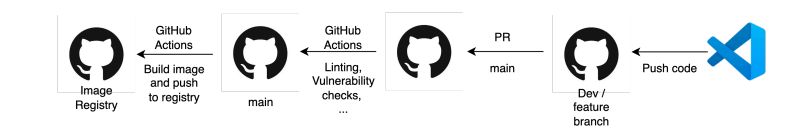
\includegraphics[width=\textwidth]{img/dev_worklfow.png}
    \caption[CI/CD-Pipeline mit GitHub Actions]{CI/CD-Pipeline mit GitHub Actions [Eigene Abbildung]}
    \label{fig:ci_cd_pipeline}
\end{figure}

Die weitere Umsetzung, wie das Pattern Continuous Deployment und Delivery in der Anwendung umgesetzt wurde, ist in \autoref{fig:infrastructure} dargestellt. Im Folgenden wird die Umsetzung kurz erläutert:

\begin{figure}[H]
    \centering
    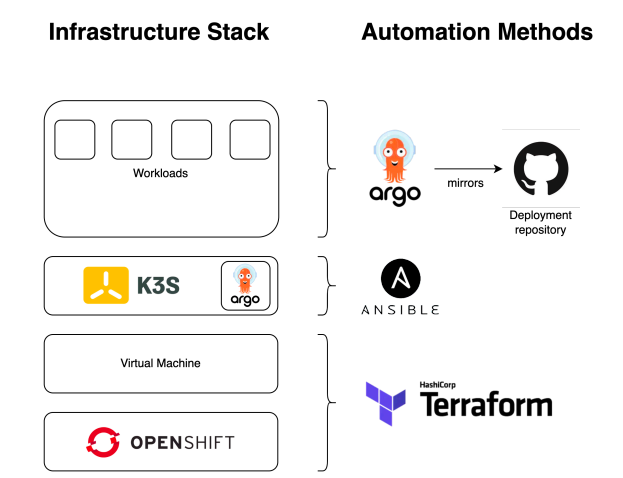
\includegraphics[width=\textwidth]{img/automation_stack.png}
    \caption[Infrastruktur der Anwendung und zugehörige Automatisierungsmethoden]{Infrastruktur der Anwendung und zugehörige Automatisierungsmethoden [Eigene Abbildung]}
    \label{fig:infrastructure}
\end{figure}

Auf der obersten Ebene befinden sich die "Workloads", die die eigentlichen Anwendungen darstellen, wie zum Beispiel das Frontend oder die einzelnen Microservices. Änderungen der Workloads, die durch eine CI-Pipeline getestet wurden, werden in ein "Deployment Repository" auf GitHub geschoben. Argo CD überwacht bzw. spiegelt dieses Repository.\\ 
Unter dieser Ebene befindet sich K3S und, eine leichtgewichtige Kubernetes-Distribution und Argo CD sowie Ansible. K3S stellt hier die Laufzeitumgebung für containerisierte Anwendungen dar. Sobald eine Änderung im Deployment Repository erkannt wird, pullt Argo CD diese Änderungen automatisch und wendet sie auf dem K3S Ziel-Cluster an. Ansible dient zur Provisionierung und zu Konfiguration der Virtual Machine, auf denen K3S läuft. Zum Beispiel wird Ansible genutzt, um neue VMs zu erstellen oder Abhängigkeiten zu konfigurieren.\\
Für die bereitstellung der Virtual Machine wird Terraform genutzt. Terraform ermöglicht es, die gesamte Infrastruktur als Code zu definieren und zu verwalten, einschließlich der Virtual Machines, auf denen OpenShift installiert wird. Dies wird ebenfalls von Terraform durchgeführt. So wird eine konsistente und reproduzierbare Infrastruktur bereitsgestellt.\\

Zusammengefasst ist die gesamte Pipeline, beginnend mit der Entwicklung, über die automatisierten Tests, bis hin zur Möglichkeit, die Anwendung und Infrastruktur in eine automatisiert zu deployen, auf Continuous Deployment und Continuous Delivery ausgelegt. Dadurch wird die Qualität der Anwendung sichergestellt, da Änderungen kontinuierlich getestet werden, und eine schnelle Reaktion auf Feedback von Nutzern sowie auf sich ändernde Anforderungen ermöglicht werden.
